\documentclass[a4paper,11pt]{article}

\parindent0cm
\usepackage
[backend=biber,style=apa,sorting=nyt]
{biblatex}
\addbibresource{literature.bib}

\usepackage[utf8]{inputenc}
\usepackage{csquotes}
\usepackage{array}
\usepackage{dirtytalk}
\usepackage{amsmath}
\usepackage{bm}
\usepackage{amssymb}
\usepackage{amsthm}
\usepackage{amsfonts}
\usepackage{color}
\usepackage{layouts}
% printing the textsize used
% \printinunitsof{cm}
% \prntlen{\textwidth}
\usepackage[usenames,dvipsnames]{xcolor}
\usepackage{tabularx}
\usepackage{graphicx}
\usepackage{pdfpages}
\usepackage[ngerman]{babel}
\usepackage[left=3cm,right=2.5cm,top=2cm,bottom=2cm]{geometry}
\renewcommand{\baselinestretch}{1.5}\normalsize % Zeilenabstand 1.5



\begin{document}

\begin{titlepage}

\vspace*{3cm}


\begin{figure}[t]
\begin{flushright}
\includegraphics[width = 7cm,  keepaspectratio]{Images/TULogo.png}


\end{flushright}
\end{figure}
\vspace*{3cm}


\begin{center}

\vspace*{2cm}

\title{Masterthesis}



{\huge Masterthesis}\\
 {\huge{\textbf{Multilabel-Klassifizierung \\
 von Nachrichten Schlagzeilen}}\\}
 \vspace{0.2cm}
 {\large  Vergleich zwischen neuronalen Netzen und baumbasierten Algorithmen auf verschiedenen Repräsentationen von Wörtern\\}
\vspace*{5cm}


{\large  Fakultät Statistik\\
Lehrstuhl Statistical Methods for Big Data }
\vspace*{0.5cm}

 \begin{large}
 Betreuer: Prof. Dr. Andreas Groll\\
  \end{large}

  \begin{large}
Verfasser: Marc Schmieder\\
\date{October 2019}
   \vspace*{2cm}

 \end{large}
\end{center}
\newpage
%\large
\thispagestyle{empty}
\tableofcontents
\newpage
\end{titlepage}







\section{Einleitung}

\begin{itemize}
    \item nutzen der klassifikation für die Redaktion
    \item oft nur binäre klassifikation, multi selteneres topic
    \item multiclass auch bei next best offer
    \item bag of words kein guten Ruf, bei welchen Datensätzen lohnen sich Neural nets überhaupt.
\end{itemize}{}

\section{Datensatz und Problemstellung}

In diesem Kapitel wird der für diese Thesis relevante Datensatz vorgestellt. Nach dessen Bereinigung erfolgt eine Exploration und anschließend die Darlegung der Zielstellung dieser Thesis.


\subsection{Initialer Datensatz}

Der Datensatz trägt den Titel \textit{News Category Dataset} (\cite{dataset}) und stammt von der Machine Learning Plattform \textit{Kaggle}. Er umfasst $200853$ Beobachtungen, die Informationen in englischer Sprache über Artikel der US-Amerikanischen Onlinezeitung \textit{Huffpost} enthalten. Der Zeitraum, in dem die Veröffentlichungen stattgefunden haben, erstreckt sich vom 28.01.2012 bis zum 25.05.2018, also über eine Zeitspanne von über $6$ Jahren. Die Inhalte der Artikel sind lediglich verlinkt und nicht direkt im Datensatz enthalten. Für jeden Artikel ist die Nachrichtenschlagzeile des Artikels angegeben. Zusätzlich zu dem Link des Artikels ist für jeden Datenpunkt das Veröffentlichungsdatum, der Name des Autors, eine Kurzbeschreibung und die Nachrichtenkategorie gegeben. Letzteres ist die Zielvariable (genauere Erläuterung in Kapitel \ref{Kap:Zielst}), die $41$ verschiedene Ausprägungen annimmt. Die Kurzbeschreibung enthält ähnliche Informationen wie die Nachrichtenüberschrift und ist nur teilweise vorhanden. Für die Beantwortung der Fragestellung (Kapitel \ref{Kap:Zielst}) soll nur die Schlagzeile als abhängige Variable in die Modellierung eingehen. Bevor eine Exploration des Datensatz erfolgt, werden im nächsten Abschnitt vorgenommene Änderungen an den relevanten Spalten Nachrichtenkategorie und Nachrichtenschlagzeile aufgelistet und begründet.


\subsection{Änderungen am Datensatz} \label{kap:2_2Aend}

In der US-amerikanischen Sprache spielt die Groß- und Kleinschreibung außer bei der Nutzung von Personalpronomen keine Rolle. Deshalb wurden in den Texten alle Großbuchstaben zu Kleinbuchstaben konvertiert. Auf diese Weise werden in der Modellierung beispielsweise die Wörter \textit{Teacher} und \textit{teacher} nicht unterschiedlich behandelt. \\
\\
Die Artikel wurden vermutlich von einigen Autoren in unterschiedlichen Ländern geschrieben, denn die Texte enthalten unterschiedliche Zeichensätze. Bei der verwendeten \texttt{utf8} Enkodierung entstanden bei unbekannten Zeichen Konvertierungsfehler (z.b. der Form \say{a@S}). Diese wurden durch Leerzeichen ersetzt. In dem Wissen, dass die Wörter des Textkorpus mit den \textit{Global Word Vectors} (Kapitel \ref{Kap:Glove}) abgeglichen werden, wurden einige Begriffe so ersetzt, dass bestimmte Wörter in den \textit{Global Word Vectors} gefunden werden. Zuerst erfolgte eine Entfernung von Sonderzeichen wie beispielsweise \say{©} oder \say{™}. Dann folgte die Ersetzung von Verneinungen wie zum Beispiel \say{n't} durch \say{ not}. Analog wurden \say{'ll} durch \say{ will} und \say{'ve} durch \say{ have} ersetzt. Kurzformen der Form \say{here's} wurden zu \say{here is} geändert, da sonst die Wörter mit Endung \say{'s} so als eigenständige Wörter repräsentiert werden und nicht sinngemäß als Tupel. Häufig vorkommende Eigennamen mit analoger Endung \say{trump's} wurden durch \say{trump his} ausgetauscht. Nachdem Vorkommnisse der Art \say{here's} entfernt worden, können nun Vorkommnisse der Art \say{john's son} durch \say{john its son} ersetzt werden. So ist bei Wörtertupeln dieser Art zwar nicht das Geschlecht von John bekannt, aber zumindest offensichtlich, dass der Sohn John zugehörig ist. Nach der Bereinigung des Textkorpus wurden letztendlich noch $6$ Schlagzeilen entfernt, die keine Wörter mehr enthalten. Es verbleiben nun also insgesamt $200847$ Beobachtungen.\\
\\
Nach der umfangreichen Bereinigung des Schlagzeilen-Textkorpuses liegt nun die Zielvariable Nachrichtenkategorie im Fokus.
Bei genauerer Betrachtung der $41$ Kategorien fällt auf, dass diese teilweise bereits namentlich sehr ähnlich ausfallen. In Tabelle \ref{tab:parentsMerge} sind beispielhaft $4$ Schlagzeilen der Kategorien \textit{parents} und \textit{parenting} aufgeführt.

\begin{table}[ht]
\begin{center}
\begin{tabular}{ | p{0.1 \textwidth} | p{0.42 \textwidth}| p{0.42 \textwidth} | }
  \hline
Beispiel & Kategorie \textit{parents}  & Kategorie \textit{parenting} \\ 
  \hline
1 & 40 tweets that sum up life with 4-year-olds & a baby book of disasters \\ 
  2 & these were the trendiest baby names in the late '80s & it is time to find your tribe \\ 
  3 & these quotes from kids are hilarious, adorable and oddly insightful & help huffpost parents win a webby award! \\ 
  4 & 30  'star wars'-inspired names parents are giving their babies & why our 'imperfect' moments are perfect to our children \\ 
   \hline
\end{tabular}
\label{tab:parentsMerge}
\caption{Beispiele für Schlagzeilen der Kategorien \textit{parents} und \textit{parenting}}
\end{center}
\end{table}

Anhand der Beispiele wird deutlich, dass es schwierig ist, diese mit menschlicher Intuition eine der beiden Kategorien eindeutig zuzuordnen. Als zusätzlicher Indikator, der für die Verschmelzung zweier Kategorien spricht, erfolgte die Betrachtung der relativen Schnittmenge der gemeinsamen häufigsten Wörter. Die häufigsten Wörter pro Kategorie wurden ermittelt, indem die kompletten Daten auf die entsprechende Kategorie gefiltert werden, anschließend Symbole und \textit{stopwords} (Wörter wie \say{he}, \say{is} oder \say{through}, die komplette Liste ist im Anhang unter (todo) zu finden) entfernt und die Wörter nach der gesamten Anzahl ihres Auftretens sortiert werden. Tabelle \ref{tab:categoryMerge} zeigt die relative Schnittmenge der $50$ häufigsten Wörter für ausgewählte Paare an Kategorien.

\begin{table}[ht]
\begin{center}
\begin{tabular}{|l|l|c|}
  \hline
Kategorie 1 & Kategorie 2  & relative Schnittmenge \\ 
  \hline
\textit{parents} & \textit{parenting} & $0.74$ \\
\textit{arts} & \textit{culture \& arts} & $0.52$\\
\textit{culture \& arts} & \textit{arts \& culture} &  $0.38$\\
\textit{arts} & \textit{arts \& culture}  & $0.40$\\
\textit{the worldpost} & \textit{worldpost} & $0.46$ \\
\textit{style} & \textit{style \& beauty} & $0.52$ \\
\textit{green} & \textit{environment} & $0.50$ \\
\hline
\textit{wellness} & \textit{black voices} & $0.16$ \\
\textit{politics} & \textit{home \& living} & $0.06$ \\
   \hline
\end{tabular}
\label{tab:categoryMerge}
\caption{Relative Schittmenge der $50$ häufigsten Wörter für Paare an Kategorien}
\end{center}
\end{table}

Die ersten $7$ Zeilen beinhalten Kategorien, die eine relative Schnittmenge von gemeinsamen Wörtern von $0.38$ oder höher haben. In den letzten beiden Zeilen ist zu sehen, dass inhaltlich verschiedene Kategorien eine vergleichbar geringe Schnittmenge an häufigsten Wörtern haben.

Mit den Argumenten der menschlichen Intuition und der Ergebnisse aus Tabelle \ref{tab:categoryMerge} wurden in folgenden Fällen die Kategorien zusammengelegt: \\
Die Kategorien \textit{parents} und \textit{parenting} wurde zu \textit{parents}, \textit{arts}, \textit{culture \& arts} und \textit{arts \& culture} zu \textit{arts \& culture}, \textit{the worldpost} und \textit{worldpost} zu \textit{worldpost}, \textit{style} und \textit{style \& beauty} zu \textit{style \& beauty} sowie \textit{green} und \textit{environment} zu \textit{green \& environment}. Beispiele analog zu \ref{tab:parentsMerge} für die anderen zusammengelegten Kategorien finden sich im Anhang (todo verlinken, auflisten). Die $41$ Kategorien wurden somit auf $35$ Kategorien reduziert, welche inhaltlich mit menschlicher Intuition unterscheidbar sind. Nach den Modifikationen folgt im nächsten Abschnitt eine Exploration des Datensatzes.

\subsection{Exploration des bereinigten Datensatzes}

Von großem Interesse ist die Verteilung der Nachrichtensparten im kompletten bereinigten Datensatz.
Abbildung \ref{abb:barplotCategories} zeigt die absoluten Anzahlen der Datenpunkte pro Nachrichtenkategorie. 

\begin{figure}[ht]
    \centering
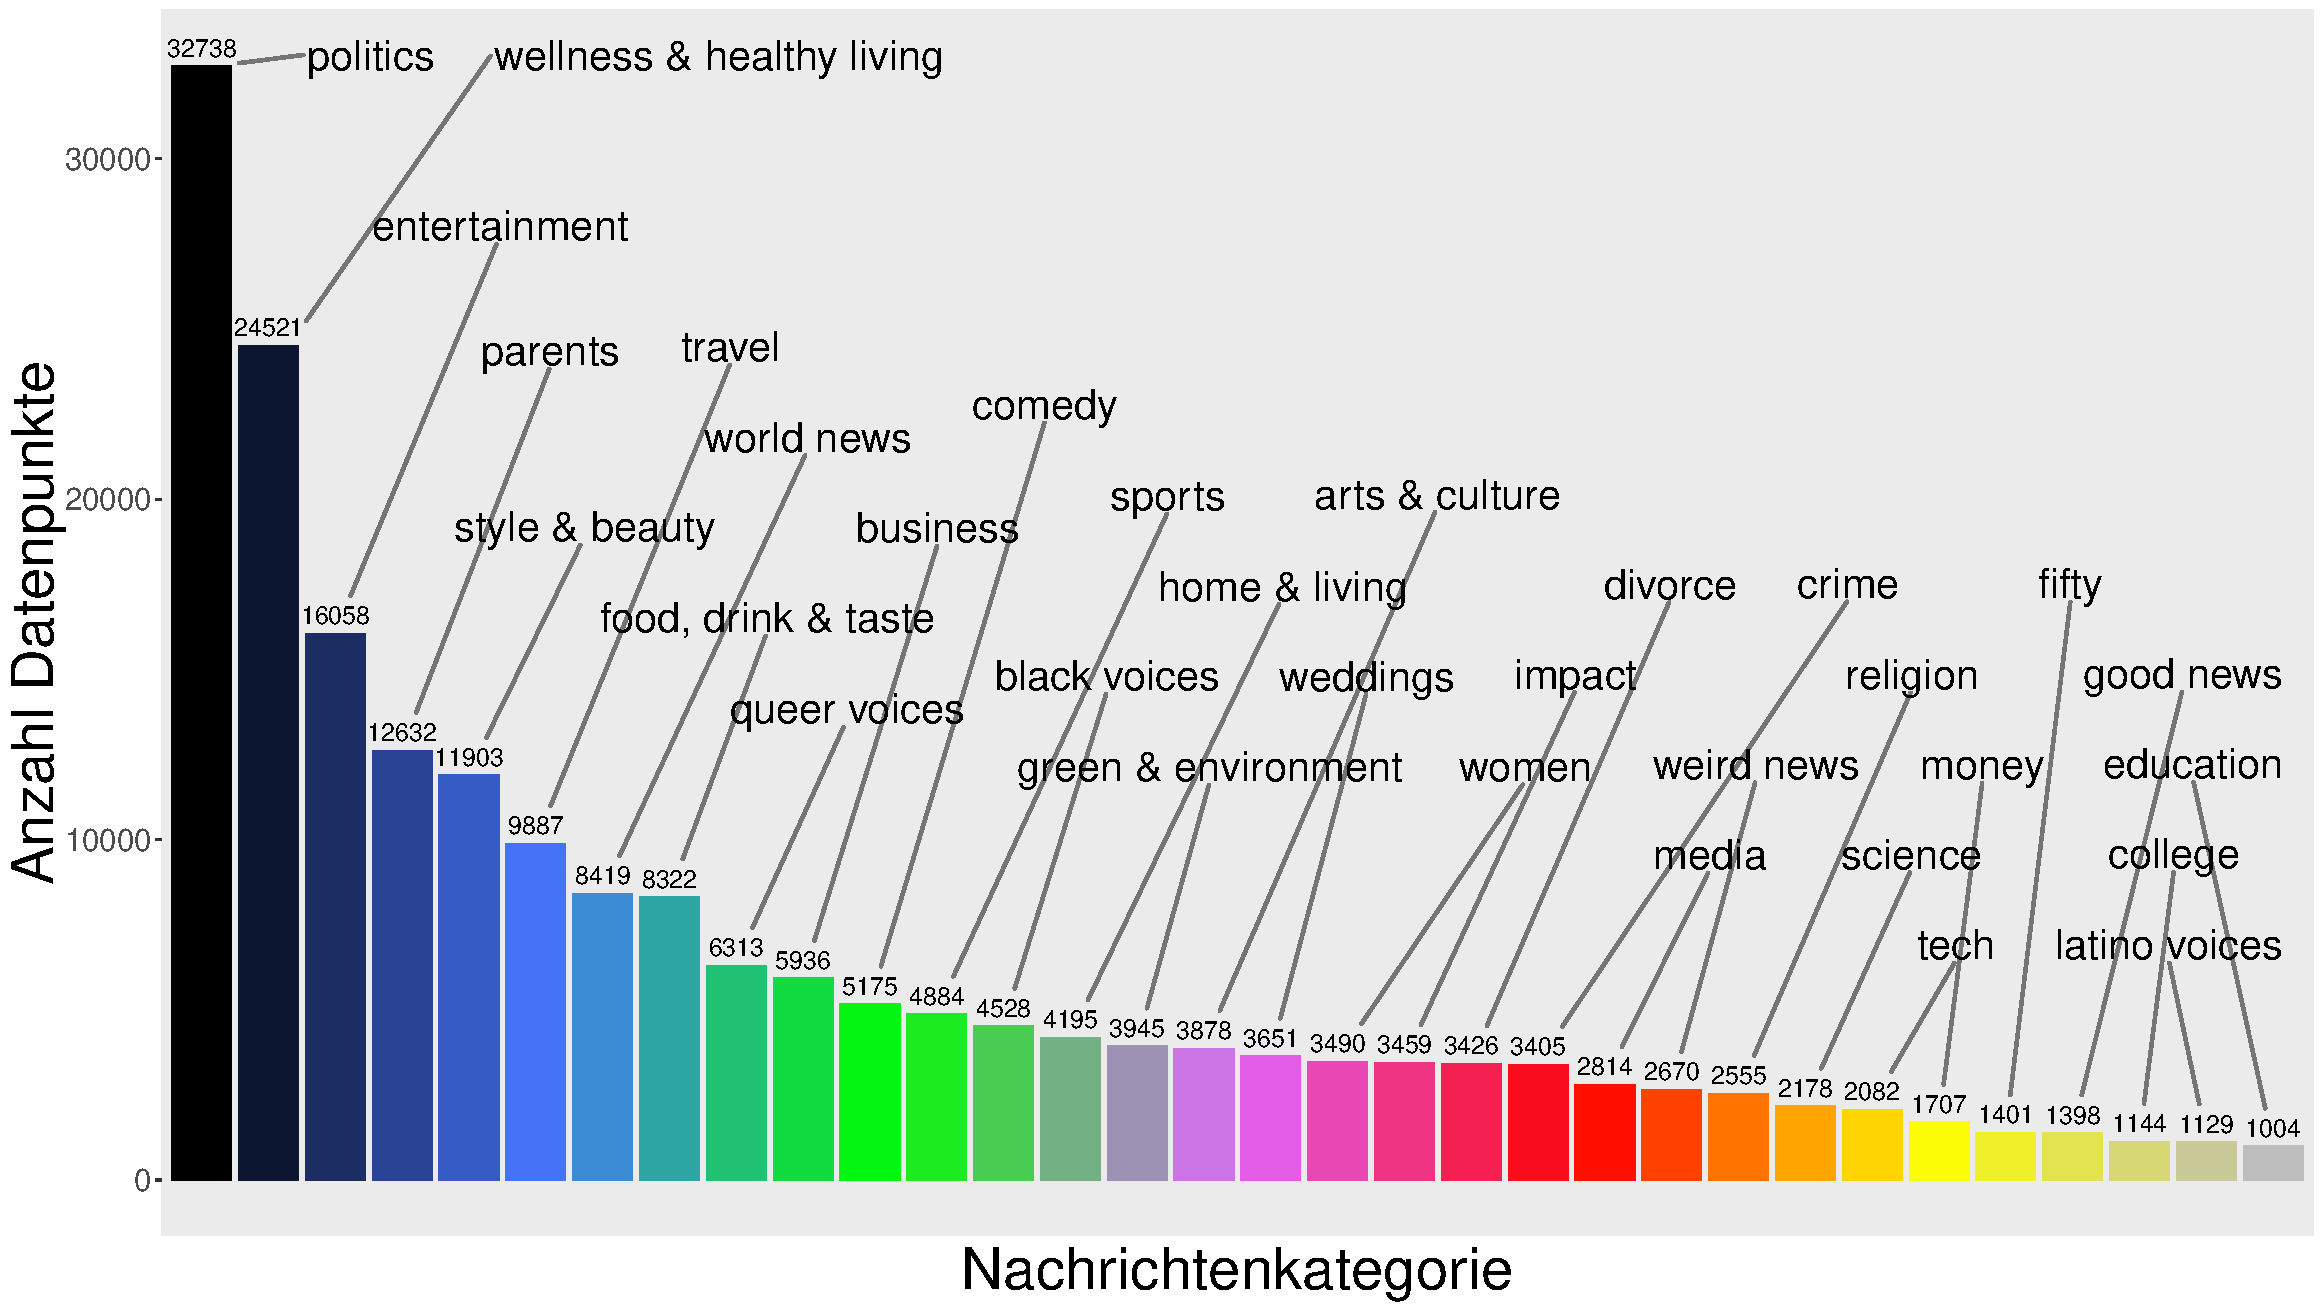
\includegraphics[width = \textwidth,  keepaspectratio]{Images/barplotCategories.pdf} 
\label{abb:barplotCategories}
\caption{Anzahl Datenpunkte pro Nachrichtenkategorie}
\end{figure}
todo: box um die labels größer machen.\\

Es ist festzustellen, dass die Kategorien keineswegs ausgeglichen vorliegen. Die häufigste Kategorie stellt \textit{politics} dar mit $32738$ Datenpunkten. Zweit- und dritthäufigste Kategorien sind \textit{wellness} und \textit{entertainment} mit $17827$ und $16058$ Beobachtungen. Die Nachrichtensparten mit den wenigsten Artikeln bilden \textit{college}, \textit{latino voices} und \textit{education} mit $1144$, $1129$ und $1004$ Beobachtungen.\\
Die ersten $6$ Kategorien stellen bereits $50.3$ Prozent der gesamten Beobachtungen dar. Durchschnittlich beinhaltet eine Kategorie $5738.5$ Nachrichtenschlagzeilen.\\
\\
Es folgt nun eine gesamtheitliche Exploration des Textkorpus der Schlagzeilen. Im Rahmen der Analyse zählen Symbole sämtlicher Art auch als Wörter. Die kürzeste Überschrift des Datensatzes enthält nur $1$ Wort, während die längste $91$ Wörter umfasst. Durchschnittlich enthält eine Schlagzeile $11.147$ Wörter. Das Vokabular aller Schlagzeilen umfasst $67938$ Wörter, wobei \say{the} das häufigste Wort ist und in $54033$ Artikelüberschriften vorkommt. $31274$ Wörter kommen nur einmal vor. In der Betrachtung der mittleren Wortanzahlen pro Kategorie fällt auf, dass diese differieren. Die Kategorie mit der höchsten durchschnittlichen Anzahl von $12.863$ Wörtern ist \textit{style \& beauty}. Die Kategorie, bei der sich die Autoren durchschnittlich am kürzesten fassen, ist \textit{food \& drink} mit $9.328$ Wörtern. Eine weitere interessante Fragestellung ist, ob in den Kategorien bestimmte Sonderzeichen oder Symbole besonders häufig oder selten vorkommen. Abbildung \ref{abb:barplotSymbols} zeigt die relative Anzahl der Vorkommnisse verschiedener Symbole in den Schlagzeilen pro Kategorie.

\begin{figure}[ht]
    \centering
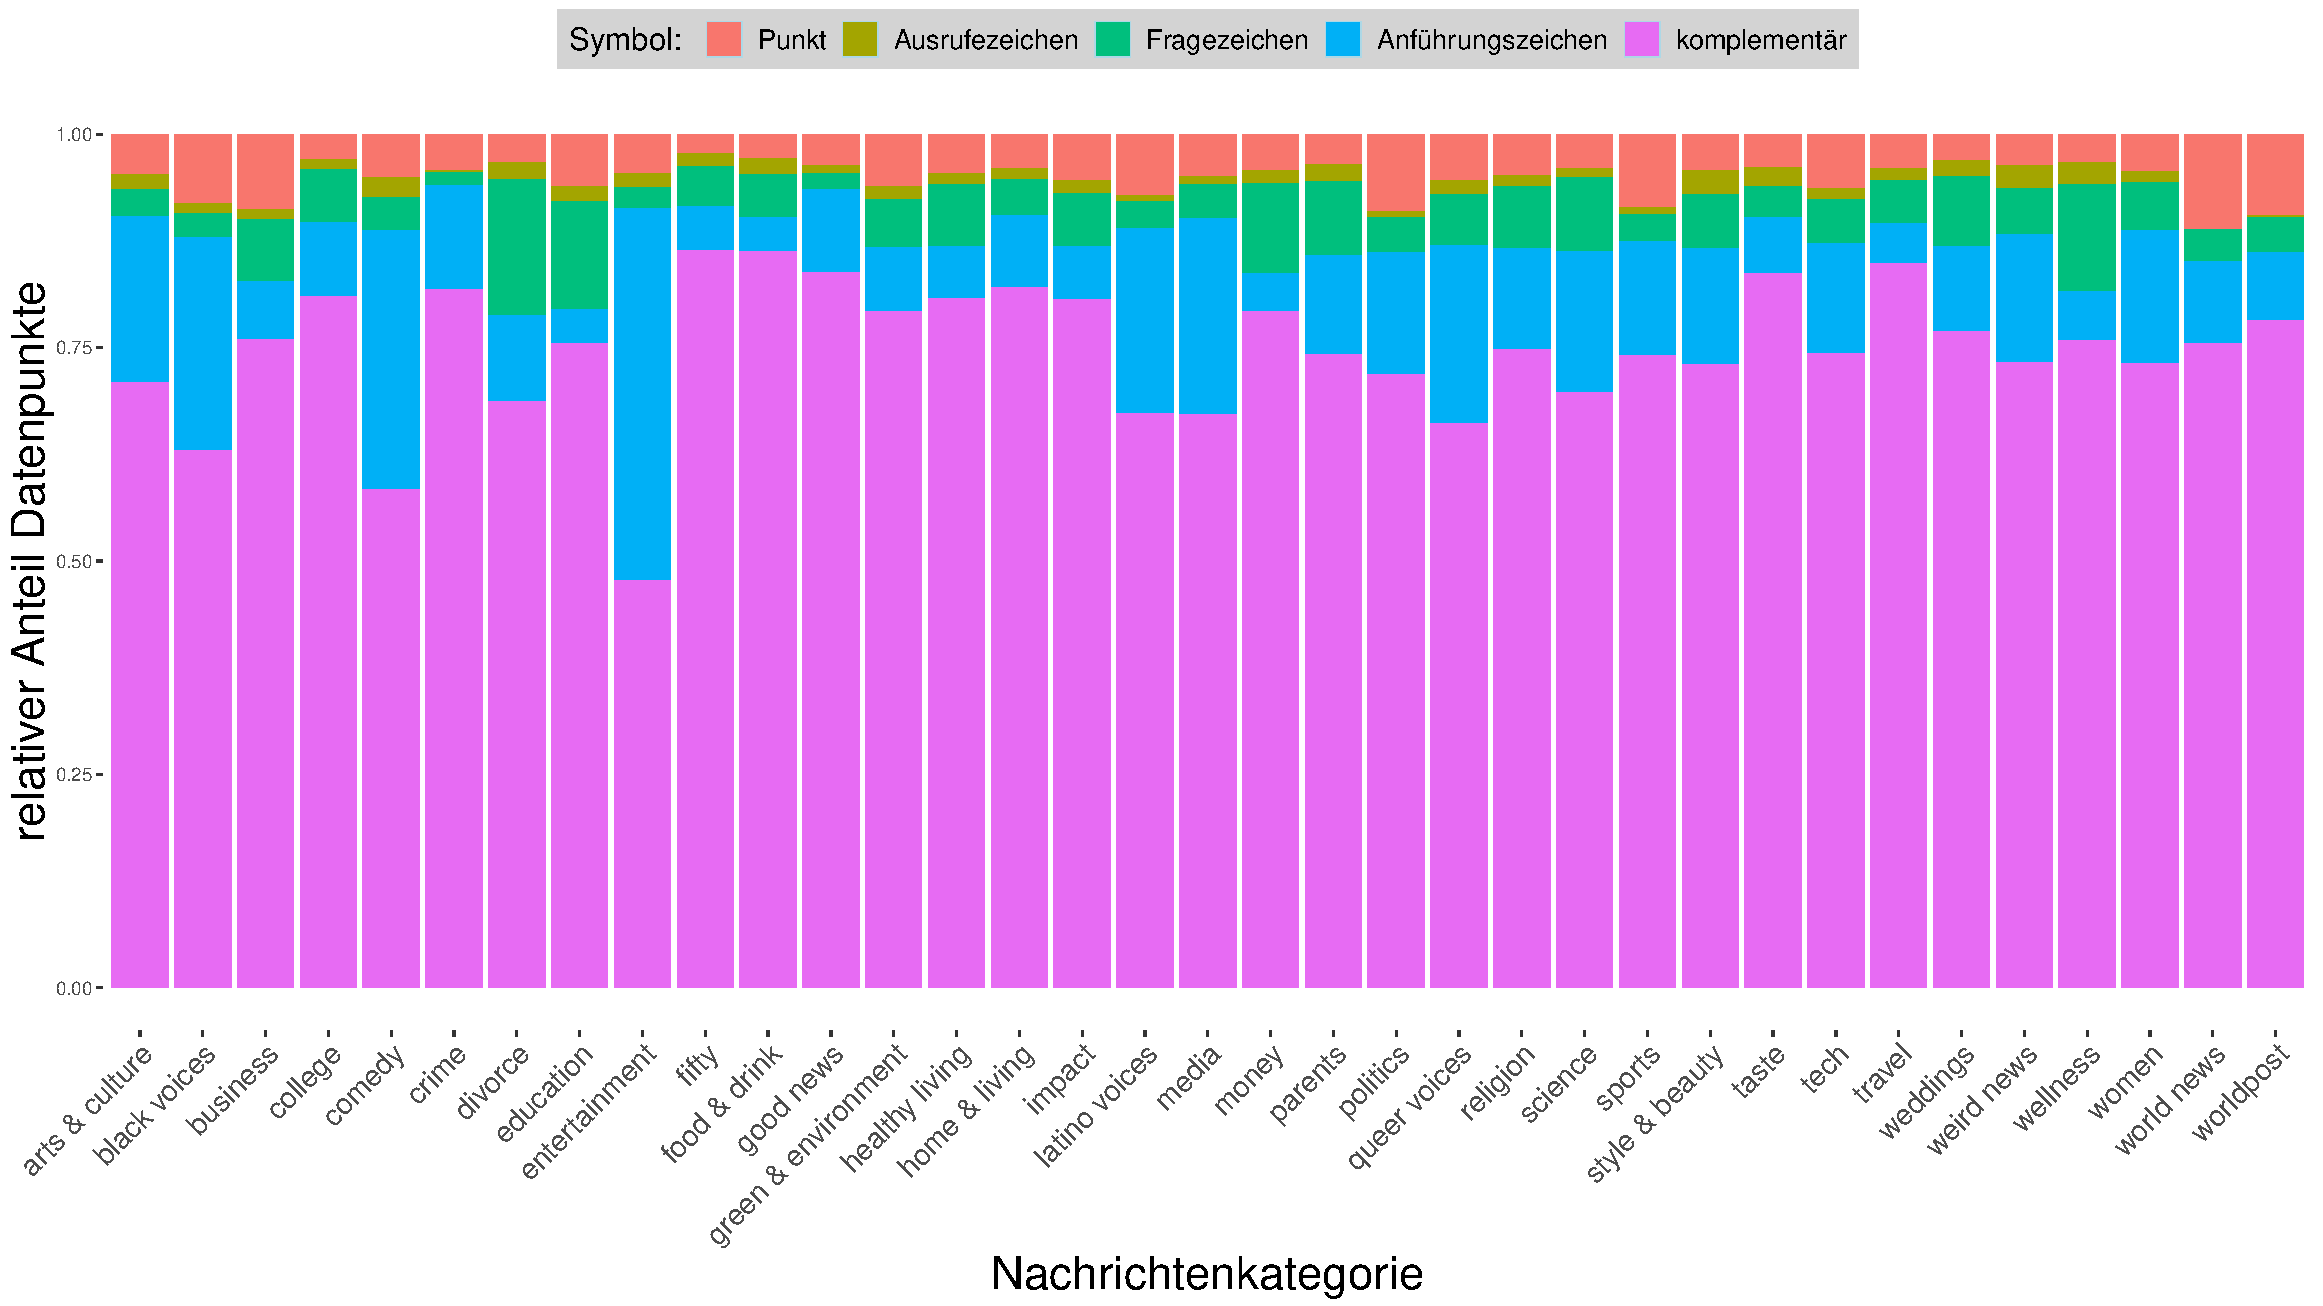
\includegraphics[width = \textwidth,  keepaspectratio]{Images/barplotSymbols.pdf} 
\label{abb:barplotSymbols}
\caption{Relativer Anteil Datenpunkte mit Sonderzeichen pro Kategorie}
\end{figure}

Ein Wert von beispielsweise $0.15$ für eine bestimmte Nachrichtensparte in der Grafik ist so zu interpretieren, dass in 15 Prozent aller Schlagzeilen dieser Kategorie das entsprechende Symbol mindestens einmal aufgetaucht ist. Die im Folgenden beschriebenen Durchschnitte sind Mittelwerte über die Kategorien und nicht über den gesamten Datensatz. Betrachtet sei nun das Vorkommen eines Punktes in einer Schlagzeile. Dieses kann so interpretiert werden, dass eine Schlagzeile 2
mehrere Sätze enthält. Dies ist insgesamt mit einem durchschnittlichen relativen Anteil von $0.051$ selten der Fall. In der Sparte \textit{world news} kommen mehrere Sätze am häufigsten vor, in \textit{fifty} am wenigsten. Der Mittelwert für Ausrufezeichen beträgt $0.014$ und die Kategorie \textit{style \& beauty} nimmt das Maximum, die Kategorie \textit{world news} das Minimum an. Fragezeichen kommen in durchschnittlich $0.059$ der Schlagzeilen vor, dabei am häufigsten in \textit{divorce} und am seltensten in \textit{crime}. Anführungszeichen sind mit durchschnittlich $0.127$ von den hier betrachteten Satzzeichen am meisten vertreten. Sie wurden besonders oft in der \textit{entertainment} Sparte genutzt und kamen am seltensten in \textit{education} zum Einsatz. Die Rubrik \say{komplementär} gibt an, zu welchem relativen Anteil keine der betrachteten Symbole vorkommt. Hier ist zu sehen, dass Kategorien wie \textit{entertainment}, \textit{comedy}, \textit{black voices} oder \textit{divorce} häufig Symbole beinhalten, die einen dramatischen Charakter ausdrücken. Sparten wie \textit{fifty}, \textit{food \& drink} und \textit{travel} bleiben mit weniger Symbolen sachlicher. Abbildung \ref{abb:barplotSymbols} zeigt insgesamt, dass Symbole für die Nachrichtensparten eine Rolle spielen und für die in Kapitel \ref{Kap:Tfidf} beschriebenen \textit{bag-of-words} und \textit{tfidf} (todo, hier entfernen, falls die Algos doch nicht genutzt werden) Ansätze nicht entfernt werden sollten.\\
\\
Es folgt nun eine Betrachtung der vorkommenden Wörter im Datensatz. Abbildung \ref{abb:WordcloudAll} zeigt eine \textit{wordcloud}, in der die häufigsten $100$ Wörter aller Kategorien (nach Entfernung von Symbolen und \textit{stopwords}) abgebildet sind.

\begin{figure}[ht]
    \centering
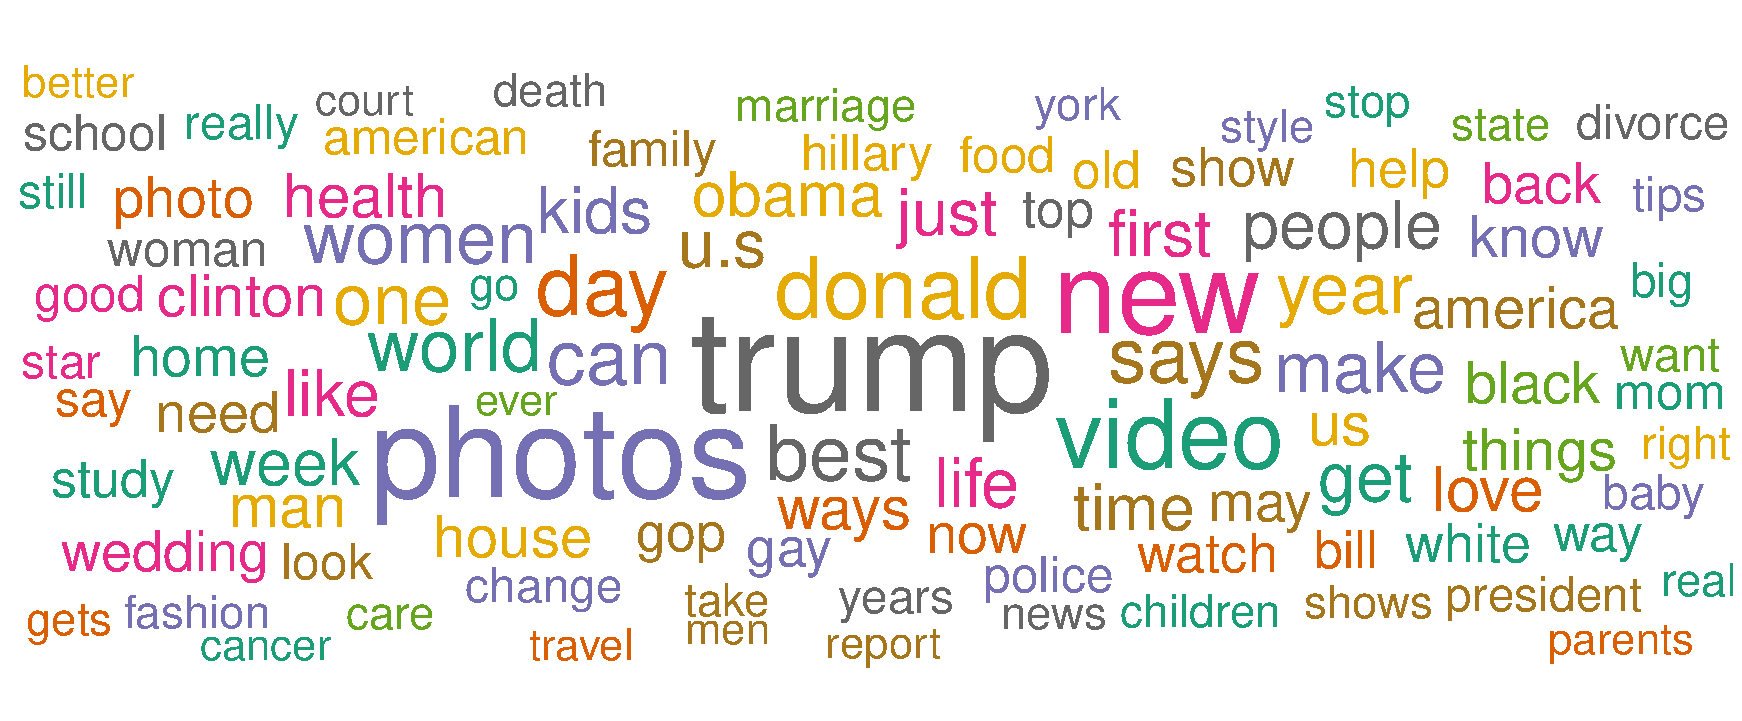
\includegraphics[width = \textwidth,  keepaspectratio]{Images/wordCloudAll.pdf} 
\label{abb:WordcloudAll}
\caption{\textit{Wordcloud} für die häufigsten 100 Wörter aller Kategorien}
\end{figure}
todo: grafik gescheit ausfüllen

Je größer ein Wort, desto häufiger kommt es insgesamt im Textkorpus vor. Es ist erstaunlich, dass \say{trump} sich über den gesamten Textkorpus als häufigstes Wort etabliert hat, in Anbetracht dessen, dass sich der Zeitraum der Daten auf über $6$ Jahre erstreckt. Die $3$ häufigsten Wörter danach sind \say{photos}, \say{new} und \say{video}. Es ist zu sehen, dass viele Namen und Begriffe aus der Politik zu sehen sind, was einleuchtend ist, da \textit{politics} zu größte Sparte darstellt. 
Auffallend ist außerdem, dass viele der auftauchenden Begriffe identisch oder fast identisch zu den Namen einiger Kategorien sind. Beispiele dafür sind \say{travel}, \say{wedding}, \say{style} oder \say{parents}. In Abbildung \ref{abb:WordcloudWellness} ist eine weitere \textit{Wordcloud} der zweitgrößten Sparte \textit{wellness} zu sehen.


\begin{figure}[ht]
    \centering
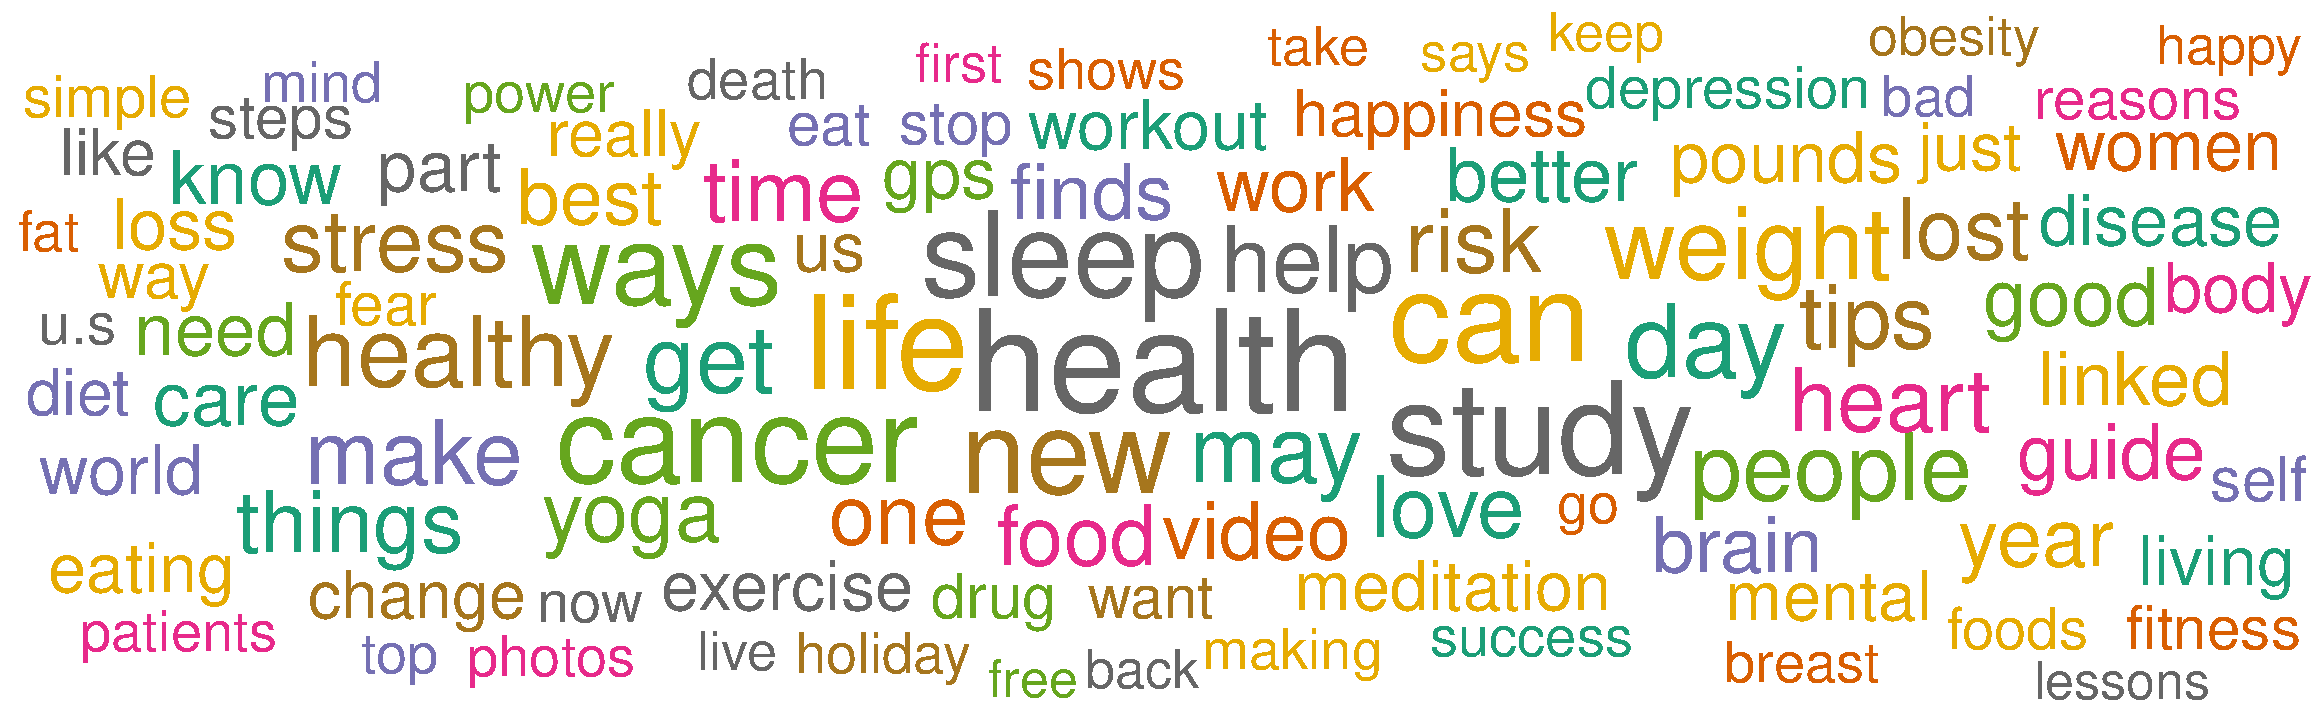
\includegraphics[width = \textwidth,  keepaspectratio]{Images/wordCloudWellness.pdf} 
\label{abb:WordcloudWellness}
\caption{\textit{Wordcloud} für die häufigsten 100 Wörter der Kategorie \textit{wellness}}
\end{figure}

In dieser Kategorie ist zu beobachten, dass oft über Schlaf, Yoga, Meditation und Sport geschrieben wird. Es werden aber auch Krankheiten wie Krebs (\say{cancer}), Übergewichtigkeit (\say{obesity}) und Diabetis angesprochen, die genauso für die Kategorie \textit{healthy living} stehen könnten. \say{yoga}, \say{breast}, \say{diet} oder \say{pounds} könnten auch legitime Schlagwörter für die \say{women} Sparte sein. Genauso ist zu vermuten, dass die Wörter \say{eat}, \say{foods} und \say{healthy} ebenso in \say{food \& drink} oft vorzufinden sind. Mit dem Blick auf die \textit{Wordclouds} und auch in Anbetracht der Kategorienzusammenlegung in Kapitel \ref{kap:2_2Aend} fällt auf, dass es nicht immer einfach ist, die Kategorien nur über ihre häufigsten Schlagwörter auseinanderzuhalten. Auf die verschiedenen Möglichkeiten, wie die Schlagzeilen in ein numerisches Datenformat überführt werden können, wird in Kapitel \ref{kap:3.1Wordemb} detailiert eingegangen.
Nachdem nun der Datensatz ausführlich exploriert wurde, folgt im nächsten Unterabschnitt die Zielstellung dieser Thesis.


\subsection{Zielstellung} \label{Kap:Zielst}

Ziel dieser Arbeit soll es sein, verschiedene Algorithmen auf verschiedenen Arten der Repräsentation der Wörter miteinander zu vergleichen. Dabei liegt ein \textit{multilabel}-Klassifikations\-problem mit $35$ Klassen vor, bei der jede Beobachtung genau einer Klasse zugehörig ist. Die Zielvariable liegt im kategoriellen Format vor. Dabei soll für die Vorhersagen $f(x_i)$ der trainierten Modelle gelten, dass
\begin{center}
$f(x_i) = p_i = (p(c_1), ...., p(c_{35}))$ \hspace{2cm} , mit $\sum\limits_{i = 1}^{35} p(c_i) = 1 $,
\end{center}
dabei sind $p(c_j)$, $j = 1,...,35$ die modellierten Wahrscheinlichkeiten der Zugehörigkeit der Beobachtung $x_i$ zur Klasse $c_j$, die in Summe $1$ ergeben müssen. Die eindeutige prognostizierte Klasse $\hat{y}$ wird dann zugeordnet durch 
\begin{center}
    $\hat{y_i} =  \underset{c_1,...,c_{35}}{argmax}$ $p(c_j)$.
\end{center}

Bezüglich der Güte der Modelle soll dann mit den Gütemaßen aus Kapitel \ref{kap:guetemass} ein Vergleich erfolgen. Dabei ist nicht nur von Interesse, wie gut die Modelle insgesamt abschneiden, sondern auch ob manche Modelle bestimmte Kategorien trennschärfer identifizieren können und welche Gründe es dafür gibt. Des Weiteren soll analysiert werden, in welche Nachbarklassen die Beobachtungen bei einer Fehlklassifikation eingeordnet werden und ob diese inhaltlich nahe an der richtigen Kategorie ist. Eine weitere Untersuchungsfrage für die Modellgüte ist, inwiefern die Repräsentation der Wörter ausschlaggebend sind und welches Gewicht der verwendete Algorithmus dabei einnimmt.
Nun sollen im nächsten Abschnitt die statistischen Methoden beschrieben werden.
(todo: diesen Abschnitt im Laufe der Arbeit ergänzen)

\newpage

\section{Statistische Methoden}

Dieses Kapitel ist in $3$ Abschnitte unterteilt. Zuerst werden die zur Bewertung der Modelle herangezogenen Gütemaße beschrieben. Es folgt die Darlegung der verschiedenen Methoden zur numerischen Repräsentation von Wörtern. Zuletzt folgt die ausführliche Beschreibung der in dieser Arbeit benutzten \textit{machine-learning} Algorithmen.

\subsection{Gütemaße zur Evaluation der Modelle}\label{kap:guetemass}

Eine Bewertung der Modelle erfolgt dann über verschiedene Kennzahlen. Einige davon werden unter Verwendung der \textit{confusion matrix} (oder auch Klassifikationsmatrix) berechnet. Diese in Tabelle \ref{tab:confusionMatrix} zu sehende Matrix stellt nach dem Anwenden des Modells auf den Testdatensatz die resultierenden Richtig- und Falschklassifikationen übersichtlich dar.

\begin{table}[ht]
\begin{center}
\begin{tabular}{|c|ccc|c|}
  \hline
 & \multicolumn{3}{|c|}{Prognostizierte Klasse} &  \\
Wahre Klasse & Kategorie $c_1$ & ...  & Kategorie $c_n$ & Zeilensumme  \\ 
  \hline
Kategorie $c_1$ & $h_{11}$ & $\hdots$ & $h_{1n}$ & $\sum_{j=1}^n h_{1j}$\\
$\vdots$ & $\vdots$ & $\ddots$ & $\vdots$ & $\vdots$ \\
Kategorie $c_n$ & $h_{n1}$ & $\hdots$ & $h_{nn}$ & $\sum_{j=1}^n h_{nj}$\\
\hline
Spaltensumme & $\sum_{i=1}^n h_{i1}$ & $\vdots$ & $\sum_{i=1}^n h_{in}$ & 
$N = \sum_{i=1}^n \sum_{j=1}^n h_{ij}$\\
   \hline
\end{tabular}
\label{tab:confusionMatrix}

  \caption{Übersicht über eine \textit{confusion matrix}  für $n$  Klassen (vgl. \cite{backhaus}, S. 238)}  
\end{center}
\end{table}

Die absoluten Häufigkeiten $h_{ij}$ stehen für die Anzahl der Beobachtungen aus der wahren Klasse $i$, für die die Klasse $j$ prognostiziert wurde. Aus der \textit{confusion matrix} können folgende Größen identifiziert werden. Die \textit{true-positives} der Klasse $i$, $tp_i = h_{ii}$ sind alle Beobachtungen, die Klasse $i$ zugehörig sind und auch in selbige Klassifiziert wurden. Die Beobachtungen, die in Klasse $i$ klassifiziert wurden, aber einer anderen wahren Klasse zugehörig sind, bezeichnet man als \textit{false-positives} $fp_i = \sum_{j = 1}^n h_{ji} - h{ii}$. Als \textit{true-negatives} $tn_i \sum_{j = 1}^n h_{ij} - h{ii}$ werden die Beobachtungen bezeichnet, die der Klasse $i$ zugehörig sind, aber in eine andere Kategorie falsch klassifiziert werden. Letztlich sind \textit{false-negatives} $fn_i = N - (tp_i + fp_i + tn_i)$ die Datenpunkte, die nicht Kategorie $i$ angehören und für die auch nicht in $i$ prognostiziert wird (vgl. \cite{sokolova}). Unter Kenntnis der 4 Häufigkeiten können nun verschiedene Gütemaße dargelegt werden. 


Die \textit{accuracy} berechnet sich analog zur binären Klassifikation aus 
\[ Acc = \frac{\sum_{i=1}^n tp_i}{N} \],
ist also der Anteil der richtig klassifizierten Beobachtungen an allen Beobachtungen. Dieses Maß ist jedoch gerade bei unbalancierten Klassifikationsproblemen nicht ideal, da große Klassen stark favorisiert werden und ein Modell schon eine hohe Güte erzielen kann, indem es alle Beobachtungen der größten Klasse zuordnet (todo quelle finden). Es folgen die Maße \textit{precision}, \textit{recall} und darauf aufbauende Kennzahlen, welche bei unterschiedlichen Klassengrößen geeigneter sind. Es wird von einer hohen \textit{precision} der Klasse $i$gesprochen, wenn nach Prognose in Klasse $i$ ein hoher Anteil dieser Beobachtungen auch tatsächlich aus derselben Kategorie stammt. Wiederum hat das Modell bezüglich Klasse $i$ einen hohen \textit{recall}, falls von den Beobachtungen der Klasse $i$ auch ein hoher Anteil in Klasse $i$ eingeordnet wird.
In der \textit{multiclass}-Klassifikation kann ein Gütemaß für das komplette Modell über \textit{micro-averaging} (mit $\mu$ indiziert) oder \textit{macro-averaging} (mit $M$ indiziert) berechnet werden. Es sind dann 
\[ precision_{\mu} = \frac{\sum_{i = 1}^n tp_i}{\sum_{i = 1}^n (tp_i + fp_i)}, \hspace{1cm} recall_{\mu} = \frac{\sum_{i = 1}^n tp_i}{\sum_{i = 1}^n (tp_i + fn_i)}\],
\[ precision_M = \frac{\sum_{i = 1}^n \frac{tp_i}{tp_i + fp_i} }{l}, \hspace{1cm} recall_M = \frac{\sum_{i = 1}^n \frac{tp_i}{tp_i + fn_i} }{l}\]
die Maße für das gesamte Modell. Ein Maß, dass \textit{precision} und \textit{recall} kombiniert ist der \textit{fscore}. Mit der unterschiedlichen Durchschnittsbildung ergeben sich
\[ fscore_{\mu} = \frac{(\beta^2+1) precision_{\mu} recall_{\mu}}{\beta^2 precision_{\mu}+ recall_{\mu}}, \hspace{1cm} fscore_{M} = \frac{(\beta^2+1) precision_{M} recall_{M}}{\beta^2 precision_{M}+ recall_{M}} \].
Hierbei ist anzumerken, dass $fscore_{\mu}$ Klassen mit vielen Beobachtungen in der Güte begünstigt während für $fscore_M$ alle Kategorien gleich wichtig sind.(todo: $beta$ spezifizieren oder multiclass AUC beschreiben).  In der statistischen Auswertung in Kapitel \ref{Kap:statAus} werden beide Kennzahlen zur Bewertung der Modelle herangezogen (vgl. \cite{sokolova}).\\

Ein weiteres Maß, um die Güte eines Multiklassifikationsproblems zu bewerten ist die kategorische \textit{cross entropy}. Diese berechnet sich aus

\[ CE = -\sum_{i=1}^N \sum_{j = 1}^n y_{ij} log(p_i(c_j)) \]

(vgl. \cite{murphy}, S.571) wobei $y_{ij} \in \{0,1\}$ indiziert, ob die Beobachtung $i$ der wahren Klasse $j$ zugehörig ist und $p_i(c_j)$ die vom Modell vorgegebene Wahrscheinlichkeit ist, dass Beobachtung $i$ zu Klasse $j$ gehört. Da $y_{ij}$ immer $0$ für alle falschen Klassen ist, entspricht $CE$ der negativen Summe der logarithmierten Wahrscheinlichkeiten der wahren Klassen über alle Beobachtungen. So wird eine geschätzte Wahrscheinlichkeit nahe $0$ für die wahre Klasse hoch und eine hohe Wahrscheinlichkeit trotz einer Fehlklassifikation weniger bestraft. Je sicherer sich das Modell für die wahren Kategorien ist, desto niedrigere Werte wird das Gütemaß annehmen (vgl. \cite{proMachine}, S. 72). 
Es gilt die \textit{cross entropy} zu minimieren. Sie nimmt ihr Minimum bei $0$ an, wenn für alle Beobachtungen eine Wahrscheinlichkeit von $1$ für die wahre Klasse prognostiziert wird.

todo: test und training eingehen.

\subsection{Repräsentationen der Wörter und Sätze (mit preprocessing der tokens} \label{kap:3.1Wordemb}

Das Extrahieren von Informationen aus Texten ist keine triviale Aufgabe, für die es viele Methoden gibt. In diesem Unterabschnitt werden einige Methoden aufgezählt, die in dieser Thesis zum Einsatz kommen.


\subsubsection{\textit{bag-of-words} und \textit{term frequency inverse document frequency}} \label{Kap:Tfidf}

Bei diesen Methoden werden zuerst für den gesamten Textkorpus ein Vokabular gebildet, das für jedes vorkommende Wort die absolute Häufigkeit des Vorkommens sowie die Anzahl der Dokumente (ein Dokument ist ein Datenpunkt, also eine Schlagzeile) enthält, in der das Wort vorkommt. Aus diesem Vokabular wird anschließend die Datenmatrix $dtm$ (\textit{document-term-matrix}) geformt, die für jede der $N$ Beobachtungen eine Zeile und für jede der $V$ Wörter eine Spalte enthält. Die Einträge der Matrix bestehen aus Werten, die das Aufkommen der Wörter beschreiben. Im simplen \textit{bag-of-words} (kurz: \textit{bow}) Ansatz ist $dtm_{ij} = f_{d_i t_j}$ die Anzahl von Wort $t_j$ in Dokument $d_i$ (vgl. \cite{deepEssentials} S. 117f). Es gibt einige Wörter wie \textit{the} oder \textit{and} die häufig vorkommen aber eventuell nicht wichtig sind. Diese \textit{stopwords} können für die \textit{bow} Methode entfernt werden. Doch generell ist dies nicht der beste Ansatz, da manche Wörter in einigen Dokumenten eine höhere Bedeutung haben können als in anderen. \\

Ein Ansatz, der diese Problematik berücksichtigt ist \textit{term frequency inverse document frequency} (kurz: \textit{tf-idf}). Hierbei werden die Gewichte $dtm_{ij}$  bei oft benutzten Ausdrücken verringert und erhöht für Wörter, die insgesamt selten benutzt werden (vlg. \cite{textMiningR} S.29). Die \textit{tf-idf} für das Dokument $d_i$ und das Wort $t_j$ berechnet sich aus 
\[tfidf(d_i, t_j) = tf(d_i,t_j) \cdot idf(t_j)  \].
Sowohl für die \textit{term-frequency} $tf$ als auch für die \textit{inverse-document-frequency} $idf$ gibt es verschiedene Berechnungsmöglichkeiten wobei in dieser Thesis folgende Formeln genutzt werden.
Die \textit{augmented-term-frequency}

\[tf(d_i,t_j) = 0.5 +  0.5 \cdot \frac{f_{d_i t_j}}{max \{ f_{d_i t_j'}: t_j' \in d_i \}} \].

berücksichtigt eine Verzerrung bei längeren Dokumenten indem durch das Maximum der vorkommenden Wörter in dem Dokument dividiert wird. Der Summand $0.5$ und Multiplikator $0.5$ dienen zur Normalisierung. Als Quotient zwischen der Anzahl der Dokumente $N$ im Korpus und der Anzahl der Dokumente die das Wort enthalten ist

\[idf(t_j) = log(\frac{N}{\# \{d_i: t_j \in d_i \}}) \]

ein geeignetes Maß (vgl. \cite{deepEssentials} S. 118). Unter Nutzung von sowohl \textit{bow} als auch \textit{tfidf} für die Repräsentation von Wörtern vernachlässigt man die Reihenfolge in den Dokumenten (vgl. \cite{deepEssentials} S. 117). Die nachfolgend beschriebenen Methoden berücksichtigen hingegegen die Reihenfolge der Wörter in einem Satz.


\subsubsection{\textit{GloVe: Global vectors for representation of words}} \label{Kap:Glove}

Eine weitere Methode zur numerischen Repräsenation von Texten sind \textit{word embeddings}, bei denen Wörter zu Vektoren fester Länge mit numerischen Werten codiert werden. Mittlerweile haben sich \textit{word embeddings} als präferierte Methode für alle Bereiche der Sprachverarbeitung im \textit{machine-learning} durchgesetzt. Die beiden bekanntesten Methoden um \textit{word embeddings} zu generieren sind \textit{word2vec} und \textit{GloVe} (vgl. \cite{keras}, S. 139). Obwohl \textit{word2vec} auf dem Lernen durch ein neuronales Netz und \textit{GloVe} auf der Zählung des Vorkommens von Wörtern im Kontext basiert, sind die beiden Verfahren von der grundsätzlichen Herangehensweise und den Resultaten ähnlich. Beide Methoden konstruieren einen Vektorraum, in dem die Position eines Worts durch den Kontext bestimmt wird, in dem das Wort im Textkorpus auftritt.
\textit{GloVe} liefert im Vergleich zu \textit{word2vec} generell etwas bessere Resultate und ist mit Paralellisierung schneller zu berechnen (vgl. \cite{keras}, S. 156). Aus diesen Gründen wird in dieser Thesis \textit{GloVe} verwendet und im Folgenden beschrieben. \\
Die Methode nutzt ein unüberwachtes Lernen zur Konstruktion der Vektoren. Zuerst wird eine Matrix $R$ konstruiert, die in den Zeilen die Wörter des Vokabulars enthält. Die Spalten enthalten ebenso die Wörter des Vokabulars, allerdings als Kontext verstanden. In den Einträgen der Matrix stehen nun die Anzahl des Vorkommens der Wörter (Zeilen) im jeweiligen Kontext (Spalten). Ob ein Wort im Kontext vorkommt, ist so zu verstehen, dass es in einem vom Anwender wählbaren Fensterbereich um das Kontextwort enthalten ist. Zur Veranschaulichung sei folgender Satz gegeben: \textit{these quotes from kids are hilarious, adorable and oddly insightful}. So kommt für einen symmetrischen Bereich von $2$ dass Wort \textit{hilarious} im Kontext von \textit{kids} einmal vor, wobei \textit{insightful} nicht im Kontext von \textit{kids} vorkommt. 
Die Matrix $R$ wird nun in das Produkt von 2 Matrizen $P$ und $Q$ zerlegt, die multipliziert eine fast identische Matrix $\Tilde{R}$ ergeben:

\begin{equation*}
\underset{N \times N}{R} = \underset{N \times F}{P} \cdot \underset{F \times N}{Q} \approx  \underset{N \times N}{\Tilde{R}} 
\end{equation*}

Die Matrix $P$ enthält in den Zeilen Wörter und in den Spalten Wort-Vektoren und die Matrix $Q$ in den Zeilen Wort-Vektoren und in den Spalten Kontext-Wörter. Sowohl $P$ als auch $Q$ werden mit zufälligen Werten gefüllt und die Matrix $\Tilde{R}$ berechnet. Mithilfe des stochastischen Gradienten-Abstieg wird nun der Inhalt von $P$ und $Q$ verändert, mit dem Ziel die Differenz zwischen $\Tilde{R}$ und $R$ zu minimieren. Dies ist ein numerischer iterativer Prozess, der wiederholt wird, bis der Fehler eine vorgegebene untere Grenze erreicht. Die Matrix $P$ enthält nun die gewünschten \textit{word-embeddings} (vgl. \cite{keras}, S. 155f). Für eine detailierte Beschreibung der Methode sei auf \cite{glovePaper} verwiesen. Die Dimension $F$ muss vom Anwender festgelegt werden. Es ist möglich diese Vektoren auf dem vorliegenden Datensatz zu trainieren, wenn der Textkorpus groß genug ist. In dem Fall des \textit{news category dataset} mit $200847$ ist dies durchaus plausibel. Das Trainieren der Vektoren erfolgte mit dem \texttt{R}-Paket \texttt{text2vec} (\cite{text2vec}) unter Verwendung der Parameter $skip\_grams\_window = 5$ für den symmetrischen Bereich des Kontextworts und die Dimension der Vektoren von $F = word\_vectors\_size = 50$.\\
Eine Alternative zum Training der \textit{word-embeddings} auf dem vorliegenden Textkorpus ist der Griff zu einem der vortrainierten Datensätze, die von \cite{gloveOnline} zur Verfügung gestellt worden. Diese Vektoren wurden auf massiven Datenmengen trainiert. Für diese Arbeit wurden 2 Datensätze mit vor-trainierten Wortvektoren des \textit{GloVe} Projekts genutzt: Ein auf Wikipedia mit $6$ Milliarden Dokumenten trainierter Datensatz mit einer Länge der Vektoren von $F = 50$ (\cite{gloveWiki}) und ein auf $42$ Milliarden aus dem Internet stammenden Textdaten mit $F = 300$ Dimensionen (\cite{gloveCommon}).\\

Allgemein haben die resultierenden Vektoren einige nützliche Eigenschaften. Als Ähnlichkeitsmaß zwischen 2 Vektoren kann das Kreuzprodukt genutzt werden. Wörter die einander ähnlich sind, sind auch im $F$-dimensionalen Vektorraum nahe beieinander angeordnet. Falls die \textit{word-embeddings} auf großen Datenmengen trainiert worden sind, können die Vektoren sogar semantische Beziehungen repräsentieren. So kann beispielsweise \textit{walking} zu \textit{walked} dieselbe Beziehung haben wie \textit{swimming} zu \textit{swam} (vlg. \cite{deepEssentials}, S. 122).


\begin{itemize}
\item R packages für Seq, tfidf und bow hinzufügen
\item erwähnen wie der Datenpunkt dann geformt wird.
\item quelle finden für summe der wort vektoren
\end{itemize}{}


\subsubsection{Sequentielle Darstellung} \label{Kap:Seq}

Eine weitere Möglichkeit, Sätze und Wörter zu repräsentieren ist als Sequenz von Indices. So bekommt jedes Wort eine natürliche Zahl aus dem Vokabular zugeordnet. Durch die Aneinanderreihung dieser Indices wird der dementsprechende Satz als Sequenz von natürlichen Zahlen dargestellt. Damit die codierten Datenpunkte jeweils die gleiche Dimension besitzen um zu einer Matrix geformt zu werden, hat jeder Vektor eine feste Länge. Dies kann die maximale Anzahl von Wörtern sein, die ein Satz enthält. Hier wurde jedoch als Kriterium $maxW$ die Anzahl Wörter genommen, die $99.9$ Prozent der News Schlagzeilen nicht überschreiten.
Da für jede Beobachtung der Vektor für die verbleibenden Wörter mit Nullen aufgefüllt wird, wird so nicht unnötig Speicherplatz verbraucht. Die resultierende Datenmatrix hat die Dimensionen $N \times maxW$. Diese kann als Trainingsdatensatz für ein klassisches \textit{machine-learning} Modell wie \textit{random Forest} dienen, oder als Input für neuronale Netze wie \textit{CNN} oder \textit{LSTM} dienen. Eine \textit{embedding} Zwischenschicht konvertiert die Indizes zu Wort Vektoren einer vorgegebenen Größe $WVSize$ und jeder Datenpunkt wird intern zu einer Matrix der Dimension $maxW \times WVSize$ während des Trainieren des Netzes gelernt. Das Bilden der Wort Vektoren geschieht in diesem Fall durch überwachtes Lernen und nicht durch unüberwachtes Lernen wie bei \textit{GloVe} in Kapitel \ref{Kap:Glove} (vgl. \cite{keras}, S.159f).\\

todo: notation der parameter checken


\subsection{Algorithmen und Verfahren}

\subsubsection{Extreme Gradient Boosting}
\subsubsection{Random Forest}

\subsection{Neuronale Netze}



\subsubsection{Multi-Layer-Perceptron Neural Net}

Dieser Abschnitt basiert größtenteils auf \cite{deepEssentials}, S.60- todo).
Das \textit{Multi-Layer-Perceptron} (kurz \textit{MLP}) ist die einfachste Form eines neuronalen Netzes. Anhand des \textit{MLP} wird im Folgenden beschrieben, wie die Struktur und die Bestandteile eines neuronalen Netzes aussehen, wie es die Parameter lernt und welche Komponenten besonders wichtig sind für die erfolgreiche Anwendung. Abbildung \ref{abb:MLPScreen} zeigt die klassifische Struktur des \textit{MLP}:


\begin{figure}[!ht]
\begin{center}
\includegraphics[width = 10cm,  keepaspectratio]{Images/MLPScreenDeepLearningEssentials.PNG}
\label{abb:MLPScreen}
\caption{\textit{fully-connected feed-forward} Netz mit 2 Zwischenschichten  (\cite{deepEssentials}, S. 60) }
\end{center}
\end{figure}

Das Netz ist organisiert in verschiedenen Schichten, die jeweils aus Neuronen (auch Knoten oder Zellen genannt) bestehen. Die Eingangsschicht (\textit{input layer}) besteht meistens aus den als numerischen Werten codierten Trainingsdaten und enthält entsprechend viele Neuronen. Darauf folgen mehrere Zwischenschichten (\textit{hidden layer}. Die Zwischenschichten können unterschiedliche Formen je nach Ziel und Architektur des Netzes haben und enthält oft eine vom Nutzer wählbare Anzahl von Neuronen. Die Ausgangsschicht (\textit{output layer}) schließt das Netz ab. Wieviele Knoten es enthält, ist abhängig von der Problemstellung. Im Falle einer Klassifikation mit $n$ Klassen enthält es ebenso viele Zellen. Nun bedeutet \textit{fully-connected}, dass jedes Neuron mit allen Neuronen aus der vorherigen und nachfolgenden Schicht verbunden ist. Die Verbindungslinien werden durch Gewichte repräsentiert, die den Einfluss des Eingangsneuron auf das Ausgangsneuron beschreiben. Bei einem \textit{feed-forward} Netz werden nur Signale in eine Richtung  zugelassen und zwar von Eingangs- bis Ausgangsschicht. Jede Schicht außer der Eingangsschicht besitzt in den Neurononen eine Aktivierungsfunktion, die bestimmt, welcher Anteil des Eingangssignal als Ausgangssignal weitergeleitet wird. Die Aktivierungsfunktion sollte differenzierbar sein, da das Netzwerk im Prozess des Lernens Gradienten berechnet. Dieser Aspekt soll später detailliert erläutert werden. Von der Vielzahl an verschiedenen Aktivierungsfunktionen werden folglich diejenigen vorgestellt, die in dieser Arbeit benutzten neuronalen Netze verwendet werden. Die \textit{rectified linear unit} (kurz \textit{relu}) hat in den letzten Jahren an Beliebtheit zugenommen.

\[\sigma(x) = 
\begin{cases}
max(0,x), & x >= 0 \\
0, & x <0
\end{cases}{}
\]

Es wurde gezeigt, dass Konvergenz unter Nutzung von \textit{relu} bis zu 6-Mal schneller erreicht werden kann. Außerdem benötigt ihre Berechnung weniger Rechenleistung als klassische Aktivierungsfunktionen. \textit{relu} wird heutzutage aus diesen Gründen in den meisten neuronalen Netzen in den Zwischenschichten verwendet. Da die Ausgangssignale nicht im Wahrscheinlichkeitsintervall $\left[0, 1\right]$ liegt, kann sie nicht für die Ausgangsschicht verwendet werden. Hierbei wird im Klassifikationsfall zur \textit{softmax} Aktivierungsfunktion gegriffen. 

\[p(y = j |z_j) = \phi(z_j) = \frac{e^{z_j}}{\sum_j^n z_j} \]

Hierbei bezeichnet $z_j$ das Ausgangssignal des Neurons der $j$-ten Klasse und $y$ die wahre Klasse. $\phi$ normiert die Ausgangssignale für jedes der $n$ Neuronen in der Ausgangsschicht und modelliert für jede der Klassen eine Art Wahrscheinlichkeit in $\left[0, 1\right]$. Insgesamt ergibt sich $\sum_{j = 1}^n \phi(z_j) = 1$. Für die in dieser Arbeit verwendeten neuronalen Netze wird jeweils eine Ausgangsschicht mit $n = 35$ Knoten gewählt und die \textit{softmax} Aktivierungsfunktion zur Transformation der Eingangssignale genutzt.\\
\\
Nachdem nun die grundlegende Architektur des Netzwerkes und die Aktivierungsfunktionen erläutert wurden, soll nun der Lernprozess durch den Gradientenabstieg und die damit verbundene Anpassung der Gewichte beschrieben werden.\\

Die Optimierung des Netzwerkes geht insofern von statten, dass die Funktion $f(x)$ bezüglich einer Verlustfunktion minimiert wird, indem $x$ geändert wird. Der Wert, der $f$ minimiert, wird notiert als 
\[x^\ast = argmin f(x)\]
Seien $x, y = f(x) \in \mathbb{R}$, so ist $f'(x) = \frac{\mathop{dx}}{dy}$ die Steigung in $x$ und gibt an, in was für einer Änderung $f(x)$ bei einer kleinen Änderung von $x$ resultiert. Unter Kenntnis von $f'(x)$ kann $f(x)$ schrittweise durch eine Änderung von $x$ in die Gegenrichtung der Ableitung minimiert werden. Diese Methode ist bekannt als Gradientenabstieg. Ist $f'(x) = 0$, so handelt es sich entweder um ein Minimum, Maximum oder einen Sattelpunkt. Ziel des Gradientenabstieg ist es, ein globales Minimum zu finden. Es ist möglich, dass die Funktion auch einige lokale Minima besitzt, die in denen $f(x)$ in einer gewissen Umgebung am kleinsten ist.


In einem Netzwerk mit 2 Zwischenschichten sei $(a_0, y)$ die Ein- und Ausgangsvektoren und $(w_1, b_1)$, $(w_2, b_2)$ die Verbindungsgewichte und \textit{bias} der Zwischenschichten. Der erste Schritt ist die Initialisierung der Gewichte und der \textit{bias} Parameter. Die Gewichte werden mit kleinen zufällige Werten initialisiert und die \textit{bias} Parameter entweder auf $0$ gesetzt oder auch mit kleinen positiven Zufallszahlen belegt (vgl. \cite{deepL}, S. 177). Eine Ausnahme stellt die Nutzung eines vortrainierten Netzes dar, das bereits gelernte Gewichte enthält. Als nächstes werden die Eingangsvektoren im Rahmen der \textit{forward-propagation} vorwärts durch das Netz geleitet. Die Berechnung erfolgt sukzessive mit
\begin{align*}
    z_1 &= a_0 \cdot w_1 + b_1 \\
    a_1 &= \sigma(z_1) \\
    z_2 &= a_1 \cdot w_2 + b_2 \\
    a_2 &= \sigma (z_2)
\end{align*}{}
$z_1, z_2$ sind die Vektoren, die in den Zwischenschichten eintreffen und $a_1, a_2$ die Signale, die die Neuronen der Zwischenschichten wieder verlassen. Anschließend wird der Fehler des Netzwerkes berechnet mit 
\[ \delta a = a_2 - y \]
oder einer anderen Kostenfunktion, die passend zum Problem ist.

\begin{itemize}
    \item backpropagation
    \item vanishing gradient problem (bei relu eingehen?
    \item batchsize/
    \item learning rate
    \item dropout
    \item batch normalization
    \item dead neurons, lieber leaky relu?
\end{itemize}{}


\subsubsection{Convolutional Neural Net}
\subsubsection{Long-Short-Term-Memory Neural Net}

\begin{itemize}
    \item grafik über kombination von word embeddings und Algorithmen (was kann mit was verwendet werden)
\end{itemize}{}


\section{Statistische Auswertung}\label{Kap:statAus}

Die Auswertung und Exploration der Daten sowie die Programmierung der Algorithmen erfolgte ausschließlich mit der Statistik-Software \texttt{R} (R Core Team, 2019).

\subsection{Framework und Vorauswahl der Verfahren}

\begin{itemize}
    \item grafik mit framework zu train/test/validation (10 prozent vorauswahl benchmarken, dann auf 90 prozent traintest/tuning. Die selben Modelle dann auf 10 prozent valdata validieren? 10 prozent war, weil dann in der kleinsten klasse noch mindestens $100$ Beobachtungen sind.
    \item außerdem welche tokens entfernt wurden.
    \item tabelle mit allem was ich ausprobiert habe
\end{itemize}{}

\subsection{Anwendung der Modelle}
\subsubsection{Performanzmaße}

\begin{itemize}
    \item accuracy, mse etc
    \item accuracy by class comparison
    \item confidence vs accuracy plots
    \item maß wie sicher ist sich das Verfahren, wenn es die richtige klasse ist?
\end{itemize}{}

\subsubsection{Explaining der besten Modelle}

\begin{itemize}
    \item beobachtungen verändern, wörter wegnehmen, hinzufügen, reihenfolge ändern und schauen ob das verfahren stabil /sensitiv zur reihenfolge
    \item nachbarklassen identifizieren
    \item convolutional filters holen und ähnlichkeiten zu combinationen aus word vectors erhalten
\end{itemize}{}

\subsubsection{Anpassung des besten Modell auf den gesamten Datensatz}

\section{Zusammenfassung}

\subsection{Ergebnisse}
\subsection{Fazit und Ausblick}

\newpage

\printbibliography[
heading=bibintoc,
title={Literaturverzeichnis}
]


\end{document}


